\section{Array x Estruturas Dinâmicas}

\begin{frame}
	\begin{block}{Array x Estruturas Dinâmicas}
		\begin{itemize}
			\item Arrays são excelentes estruturas de dados, infelizmente tem tamanho fixo. Essa limitação nos obriga a saber o tamanho total a ser alocado previamente ou devemos copiar o array para um array maior sempre que o tamanho estourar.

			\item Para evitar esse problema existem estruturas de dados dinâmicas. Onde não há necessidade de alocar memória previamente ou recopiar a estrutura toda para uma nova. Elas crescem a medida que tamanho é solicitado
		\end{itemize}
	\end{block}
\end{frame}

\section{Lista Ligada - 1 encadeamento}
\begin{frame}
	\begin{block}{Lista Ligada - 1 encadeamento}
		\begin{itemize}
			\item A primeira estrutura de dados dinâmica que iremos estudar é a lista ligada com encadeamento simples.
	
			\item Consiste em um conjunto de nós, cada nó armazena dados e um ponteiro com a posição em memória do próximo nó.
			
			\item Cada novo nó a estrutura aloca memória extra para ele e encadeia no restante da lista.
			
			\item No início a lista é vazia com apenas um ponteiro para NULL, ao adicionar o primeiro nó, alocamos memória e fazemos o último nó da lista apontar para o novo nó.
		\end{itemize}
	\end{block}
\end{frame}

\begin{frame}
	\begin{block}{Lista Ligada - 1 encadeamento}
		\begin{figure}[!htb]
			\centering	  				
			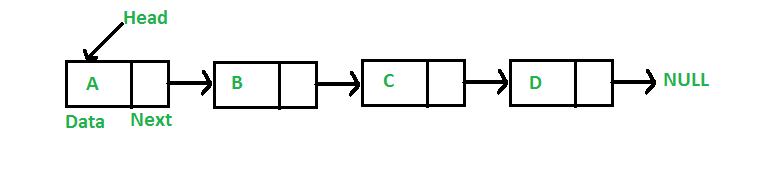
\includegraphics[height=3cm, width = 9cm]{./pic/LinkedlistUmEncadeamento.png}
			\caption{Lista Ligada - 1 encadeamento \cite{GEEKS_2018}}
			\label{fig_LLS_one}
		\end{figure}
	\end{block}
\end{frame}

\begin{frame}
	\begin{block}{Lista Ligada - 1 encadeamento: Inserção}
	\begin{itemize}
			\item A primeira estrutura de dados dinâmica que iremos estudar é a lista ligada com encadeamento simples.
	
			\item Há três casos para inserção, variando de acordo com a posição do nó na lista: 
			
			\item Novo head 
			
			\item Entre nós
			
			\item Último nó da lista
		\end{itemize}
	\end{block}
\end{frame}

\begin{frame}
	\begin{block}{Lista Ligada - 1 encadeamento: Inserção}
		\begin{figure}[!htb]
			\centering	  				
			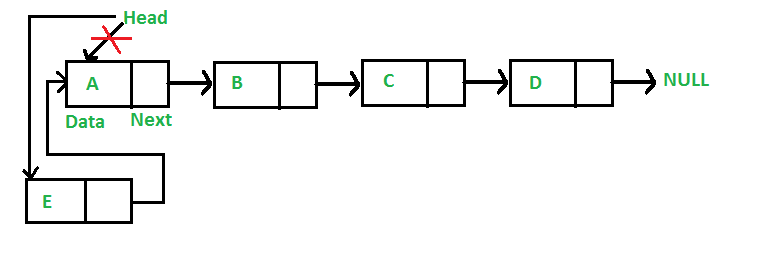
\includegraphics[height=3cm, width = 9cm]{./pic/Linkedlist_insert_at_start.png}
			\caption{Lista Ligada - 1 encadeamento: Inserção no início \cite{GEEKS_2018}}
			\label{fig_LLS_two}
		\end{figure}
	\end{block}
\end{frame}

\begin{frame}
	\begin{block}{Lista Ligada - 1 encadeamento: Inserção}
		\begin{figure}[!htb]
			\centering	  				
			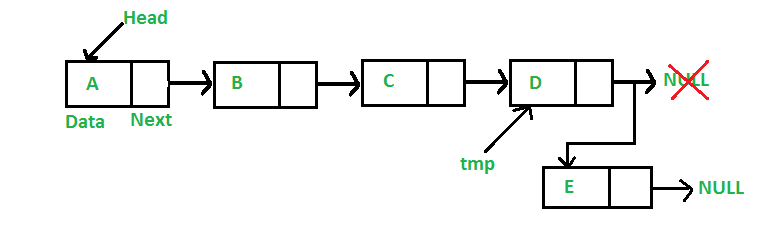
\includegraphics[height=3cm, width = 9cm]{./pic/Linkedlist_insert_last.png}
			\caption{Lista Ligada - 1 encadeamento: Inserção no fim \cite{GEEKS_2018}}
			\label{fig_LLS_three}
		\end{figure}
	\end{block}
\end{frame}

\begin{frame}
	\begin{block}{Lista Ligada - 1 encadeamento: Inserção}
		\begin{figure}[!htb]
			\centering	  				
			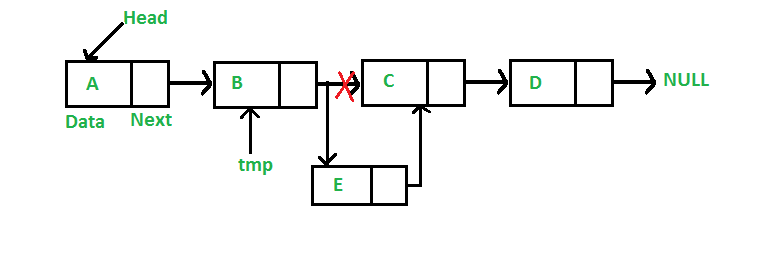
\includegraphics[height=3cm, width = 9cm]{./pic/Linkedlist_insert_middle.png}
			\caption{Lista Ligada - 1 encadeamento: Inserção no meio \cite{GEEKS_2018}}
			\label{fig_LLS_four}
		\end{figure}
	\end{block}
\end{frame}


\begin{frame}

	\begin{block}{Lista Ligada - 1 encadeamento: Deleção}
		\begin{itemize}
			\item O anterior aponta para o next do nó deletado
		\end{itemize}
		\begin{figure}[!htb]
			\centering	  				
			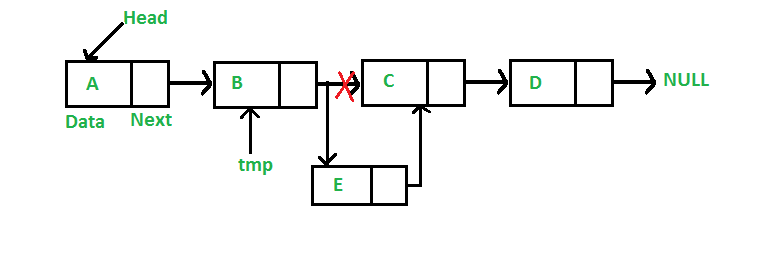
\includegraphics[height=3cm, width = 9cm]{./pic/Linkedlist_insert_middle.png}
			\caption{Lista Ligada - 1 encadeamento: Inserção no meio \cite{GEEKS_2018}}
			\label{fig_LLS_five}
		\end{figure}
	\end{block}
\end{frame}

\begin{frame}
	\begin{block}{Lista Ligada}
	\begin{itemize}
			\item Programar com os alunos em C\#
			\item Mostrar complexidade
		\end{itemize}
	\end{block}
\end{frame}

\section{Lista Ligada - 2 encadeamentos}
\begin{frame}
	\begin{block}{Lista Duplamente Ligada}
	\begin{itemize}
			\item As listas duplamente encadeadas seguem o mesmo raciocínio de listas encadeadas simples... São estruturas dinâmicas que permitem flexibilidade na criação de novos elementos.

			\item Possuem como  diferencial um encadeamento extra para o nó anterior além do seguinte. Isso permite percorrer com facilidade os nós da lista em ambos os sentidos.
		\end{itemize}
	\end{block}
\end{frame}

\begin{frame}
	\begin{block}{Lista Duplamente Ligada}
		\begin{figure}[!htb]
			\centering	  				
			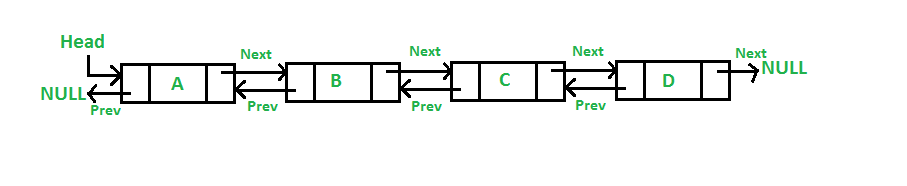
\includegraphics[height=3cm, width = 9cm]{./pic/DLL1.png}
			\caption{Lista Ligada - 1 encadeamento: Inserção no meio \cite{GEEKS_2018}}
			\label{fig_LLS_six}
		\end{figure}
	\end{block}
\end{frame}

\begin{frame}
	\begin{block}{Lista Duplamente Ligada: Inserção}
	\begin{itemize}
			\item Há quatro casos para inserção, variando de acordo com a posição do nó na lista: 

			\item Novo head 
			
			\item Após um nó
			
			\item Antes de um nó
			
			\item Último elemento da lista
		\end{itemize}
	\end{block}
\end{frame}



\begin{frame}
	\begin{block}{Lista Duplamente Ligada: Inserção}
		\begin{figure}[!htb]
			\centering	  				
			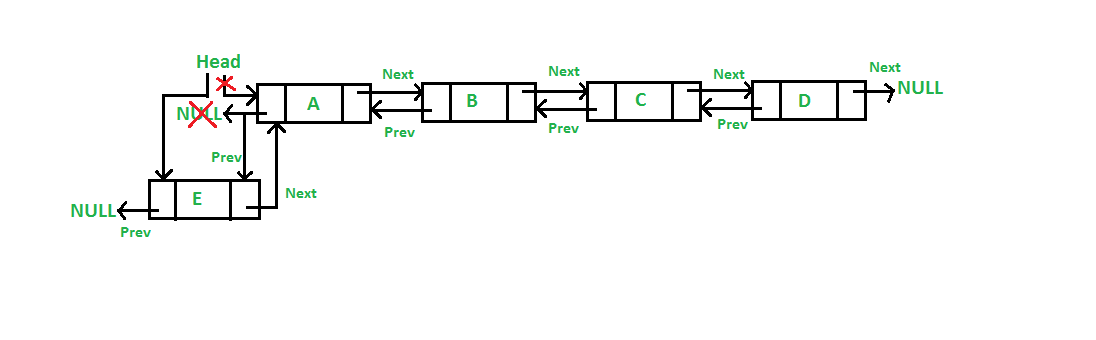
\includegraphics[height=3cm, width = 9cm]{./pic/DLL_add_front1.png}
			\caption{Lista Ligada - 1 encadeamento: Inserção na frente \cite{GEEKS_2018}}
			\label{fig_LDE_front}
		\end{figure}
	\end{block}
\end{frame}


\begin{frame}
	\begin{block}{Lista Duplamente Ligada: Inserção}
	\begin{itemize}
			\item Após "B"
	\end{itemize}
		\begin{figure}[!htb]
			\centering	  				
			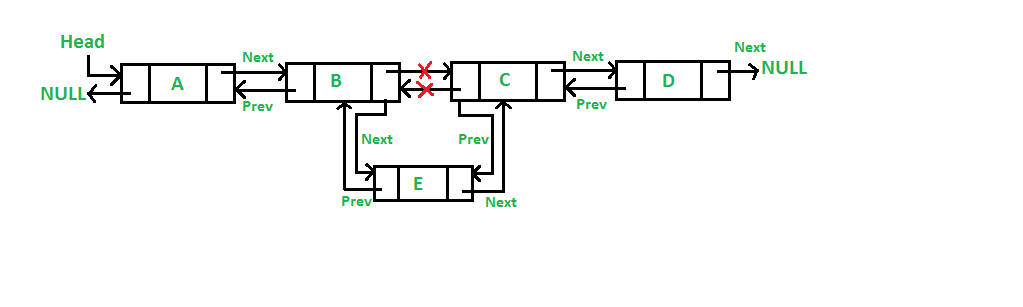
\includegraphics[height=3cm, width = 9cm]{./pic/DLL_add_middle1.png}
			\caption{Lista Ligada - 1 encadeamento: Inserção no meio \cite{GEEKS_2018}}
			\label{fig_LDE_midle1}
		\end{figure}
	\end{block}
\end{frame}


\begin{frame}
	\begin{block}{Lista Duplamente Ligada: Inserção}
	\begin{itemize}
			\item Antes de "C"
	\end{itemize}
		\begin{figure}[!htb]
			\centering	  				
			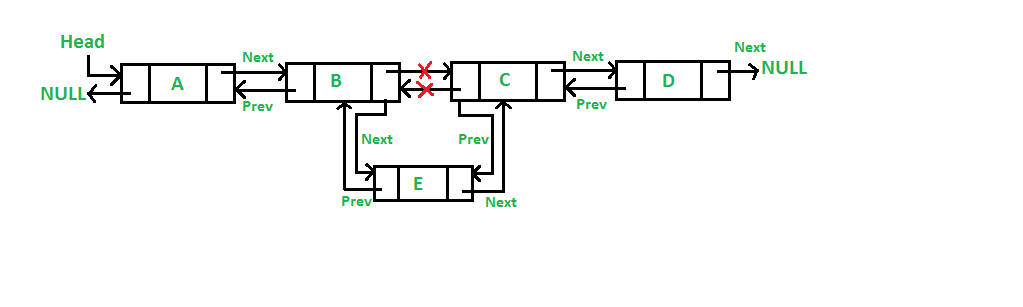
\includegraphics[height=3cm, width = 9cm]{./pic/DLL_add_middle1.png}
			\caption{Lista Ligada - 1 encadeamento: Inserção no meio \cite{GEEKS_2018}}
			\label{fig_LDE_midle2}
		\end{figure}
	\end{block}
\end{frame}


\begin{frame}
	\begin{block}{Lista Duplamente Ligada: Inserção}
		\begin{figure}[!htb]
			\centering	  				
			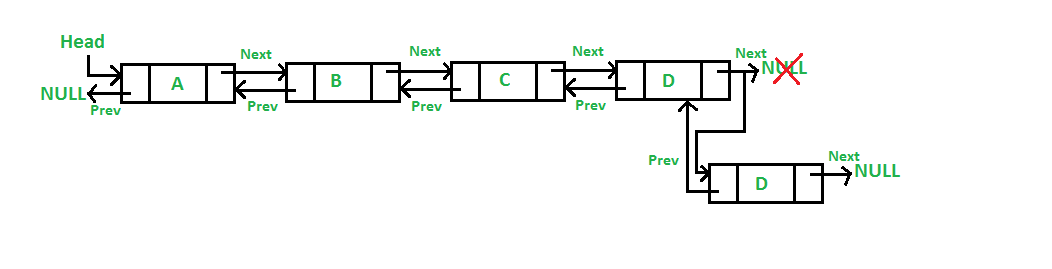
\includegraphics[height=3cm, width = 9cm]{./pic/DLL_add_end1.png}
			\caption{Lista Ligada - 1 encadeamento: Inserção no fim \cite{GEEKS_2018}}
			\label{fig_LDE_end}
		\end{figure}
	\end{block}
\end{frame}



\begin{frame}
	\begin{block}{Lista Duplamente Ligada: Deleção}
		\begin{figure}[!htb]
			\centering	  				
			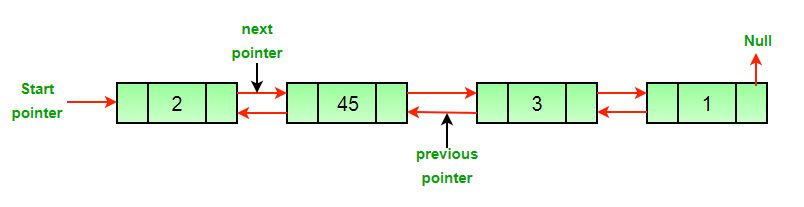
\includegraphics[height=3cm, width = 9cm]{./pic/Delete_lincked_list.jpg}
			\caption{Lista Ligada - 1 encadeamento: Deleção \cite{GEEKS_2018}}
			\label{fig_LDE_end}
		\end{figure}
	\end{block}
\end{frame}


\begin{frame}
	\begin{block}{Lista Duplamente Ligada: Deleção}
		\begin{figure}[!htb]
			\centering	  				
			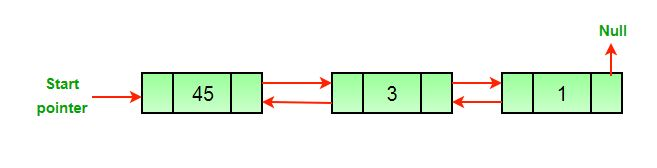
\includegraphics[height=3cm, width = 9cm]{./pic/Delete_lincked_list2.jpg}
			\caption{Lista Ligada - 1 encadeamento: Deleção \cite{GEEKS_2018}}
			\label{fig_LDE_end}
		\end{figure}
	\end{block}
\end{frame}


\begin{frame}
	\begin{block}{Lista Duplamente Ligada: Deleção}
		\begin{figure}[!htb]
			\centering	  				
			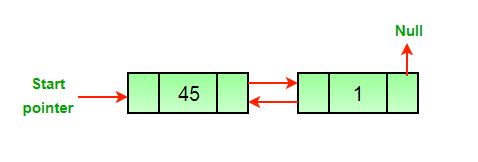
\includegraphics[height=3cm, width = 9cm]{./pic/Delete_lincked_list3.jpg}
			\caption{Lista Ligada - 1 encadeamento: Deleção \cite{GEEKS_2018}}
			\label{fig_LDE_end}
		\end{figure}
	\end{block}
\end{frame}

\begin{frame}
	\begin{block}{Lista Duplamente Ligada: Deleção}
		\begin{figure}[!htb]
			\centering	  				
			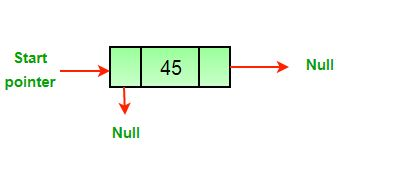
\includegraphics[height=3cm, width = 9cm]{./pic/Delete_lincked_list4.jpg}
			\caption{Lista Ligada - 1 encadeamento: Deleção \cite{GEEKS_2018}}
			\label{fig_LDE_end}
		\end{figure}
	\end{block}
\end{frame}

\begin{frame}
	\begin{block}{Lista Duplamente Ligada}
	\begin{itemize}
			\item Programar com os alunos em C\#
			\item Mostrar complexidade
		\end{itemize}
	\end{block}
\end{frame}

\section{Lista Ligada - Circular}
\begin{frame}
	\begin{block}{Lista Circular}
	\begin{itemize}
			\item Listas ligadas podem ser circulares, onde o último nó aponta para o primeiro ao invés de apontar para: "null"

			\item Normalmente usadas para implementar filas
			
			\item Usadas pelo OS para alocar recursos por um período de tempo

		\end{itemize}
	\end{block}
\end{frame}

\begin{frame}
	\begin{block}{Lista Circular}
	\begin{itemize}
			\item O nó, operações de deleção e inserção são como no caso da lista simples usando os nós de head e tail para gerenciar a lista.
	\end{itemize}
		\begin{figure}[!htb]
			\centering	  				
			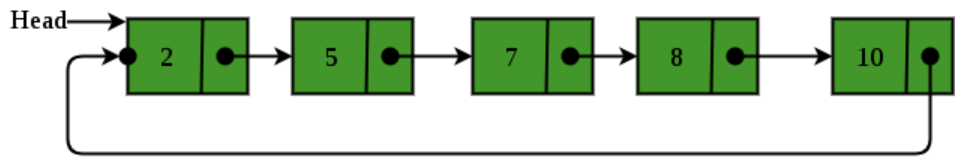
\includegraphics[height=3cm, width = 9cm]{./pic/ListaCircular.png}
			\caption{Lista Circular \cite{GEEKS_2018}}
			\label{fig_LDE_midle2}
		\end{figure}
	\end{block}
\end{frame}

\begin{frame}
	\begin{block}{Lista Circular}
	\begin{itemize}
			\item Programar com os alunos em C\#
			\item Mostrar complexidade
		\end{itemize}
	\end{block}
\end{frame}
